\documentclass[12pt]{article}

\usepackage[utf8]{inputenc}
\usepackage{polski}
\usepackage{indentfirst} %wcienia od pierwszego akapitu
\usepackage{amsfonts}    %czcionki np funkcja do pogrubienie dla np N
\usepackage{amsmath} %zawiera np begin cases
\usepackage[dvipsnames]{xcolor} %kolory dvipsnames wiecej kolor�w
\usepackage{graphicx} %np includeggraphics do obrazkow
\usepackage{caption} %np caption czyli podpisy pod obrazkiem
\usepackage{epstopdf} %np do obrazki wektorowe na pdf
\usepackage{scrextend}
\usepackage{geometry} %zmienia marginesy
\usepackage{fancyhdr}
\usepackage{lastpage}
\usepackage{wrapfig}
\usepackage{subcaption}
\usepackage{amssymb}
\usepackage{mathtools}
\usepackage{enumitem}
\usepackage{subcaption}
\usepackage{caption}
\usepackage{multicol}
\usepackage{listings}

\begin{document}

\newgeometry{margin=0.7in}
\begin{flushright}
\textbf{Wydział:} Fizyki i Informatyki Stosowanej\\
\textbf{Kierunek:} Informatyka Stosowana\\
\textbf{Rok:} 2022/23\\
\textbf{Semestr}: zimowy\\
\textbf{Typ:} stacjonarne\\
\textbf{Nr albumu:} 401984\\
\textbf{Data:} 20.11.2022\\
\end{flushright}

\begin{center}

\includegraphics[scale=0.15]{AGH}
\\[0.3cm]
\begin{LARGE}
\textsf{Dokumentacja Projektu Flight Planner\\
Przetwarzanie danych w chmurach obliczeniowych
\\[1cm]}
\end{LARGE}
\end{center}

\tableofcontents
\vspace*{\fill}

\begin{LARGE}
\begin{flushleft}
{\Large opracował:\\
Tomasz Szkaradek\par}
\end{flushleft}
\end{LARGE}

\clearpage
\newpage
\restoregeometry
\cfoot{\thepage\ of \pageref{LastPage}}
\newgeometry{margin=1in}

\section{Opis projektu, koncepcji i założeń}
Tematem projektu jest "Fight Planner" który umożliwia użytkownikowi zarządzanie swoimi podróżami, pozwala też na organizacje infrastruktury lotnisk na świecie. Aplikacja zawiera opcje do znajdywania najkrótszej ścieżki między skomunikowanymi lotniskami albo ścieżkę z najmniejszą liczbą przesiadek.\\
Lista możliwości, jakie zapewnia aplikacja/API:
\begin{itemize}
    \item Dodanie nowego lotniska do bazy
    \item Edycja wybranego lotniska
    \item Usuniecie danego lotniska z bazy
    \item Dodanie połączenia z wybranym lotniskiem
    \item Wyszukanie lotniska po wybranym parametrze
    \item Otrzymanie listy wszystkich dostępnych lotnisk
    \item Wyszukanie połączenia po nazwie miasta
    \item Otrzymanie listy wszystkich połączeń
    \item Wyszukanie najkrótszej ścieżki pomiędzy lotniskami
    \item Wyszukanie ścieżki z najmniejszą liczbą wezłów pomiędzy lotniskami
\end{itemize}
\begin{figure}[!ht]
    \begin{subfigure}{.5\linewidth}
        \centering
        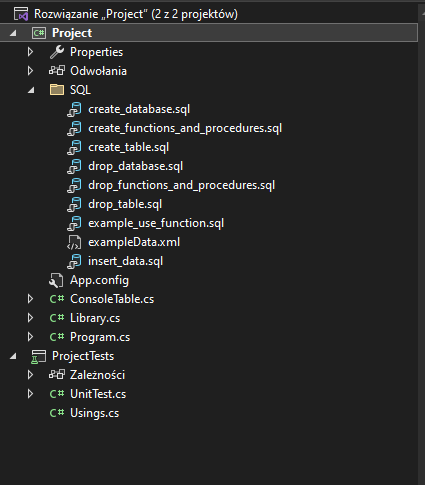
\includegraphics[width=0.95\linewidth]{6} 
        \caption{Formularz dodawania połączenia}
    \end{subfigure}
    \begin{subfigure}{.5\linewidth}
        \centering
        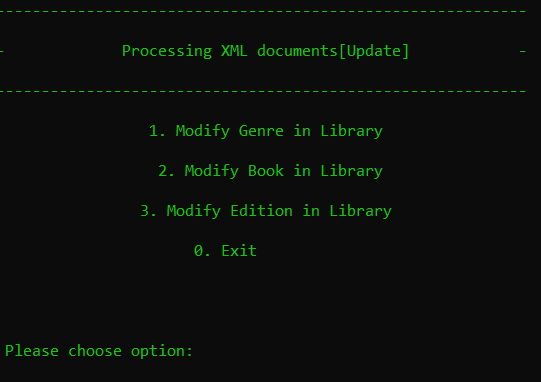
\includegraphics[width=0.95\linewidth]{8}  
        \caption{Najkrótsza ścieżka miedzy Warszawą a Bogotą}
    \end{subfigure}
\end{figure}
\newpage
\section{Krótki opis architektury}
Aby zaprezentować przepływ danych w aplikacji skonstuowany został diagram sekwencji
\begin{figure}[!ht]
    \centering
    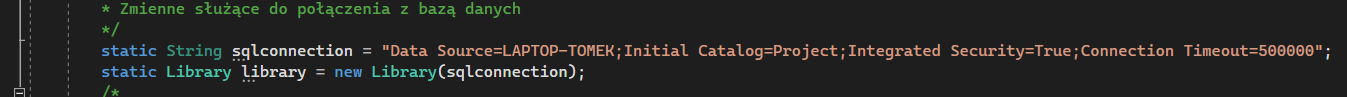
\includegraphics[width=0.95\linewidth]{10}  
    \caption{Diagram sekwencji funkcjonalności}
\end{figure}
\section{Zastosowane narzędzia i technologie}
Aplikacja została podzielona na część frontendową napisaną w języku JavaScript wykorzystując technologie React oraz bibliotekę Bootstrap. Natomiast w części backendowej aplikacji różnież wykorzystano język JavaScript oraz bibliotekę express z ich pomocą stworzono
REST API zdolne zapisywać dane przesłane jako żądanie POST w postaci JSON-a oraz obsłużyć żądania takie jak GET/PUT/DELETE.
Baza danych przechowywana jest na chmurowym rozwiązaniu Aura DB dla Neo4j, a zapytania do niej konstruowana są przy pomocy dedykowanego języka Cypher.
\newpage
\section{Reprezentacja grafowa}
Na poniższym zdjęciu możemy zobaczyć strukturę grafową z postaci grafu skierowanego naszej bazy danych.
Wierzchołkami w tym grafie są poszczególne lotniska natomiast występujące między nimi krawędzie/relacje to połączenie skierowane (skierowanie wskazuje lotnisko startowe i lotnisko docelowe) 
\begin{figure}[!ht]
    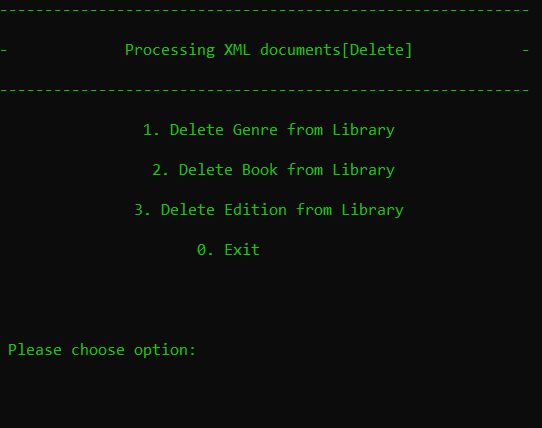
\includegraphics[width=0.99\linewidth]{9}  
    \caption{Reprezentacja grafowa lotnisk i połączeń}
\end{figure}
\newpage
\section{Prezentacja działania aplikacji}
Projekt dostarcza dwie podstawowe funkcjonalności z poziomu interfejsu
użytkownika: 
\begin{itemize}
    \item Zarządzanie lotniskami
    \item Zarządzanie/wyszukiwanie optymalnych połączeń
\end{itemize}
Na początku musimy zarejestrować się do naszej aplikacji.Wypełniając formularz wysyłany jest kod aktywacyjny na podany mail, a następnie tworzone jest nasze konto, do którego możemy się zalogować.\\
\begin{figure}[!ht]
    \centering
    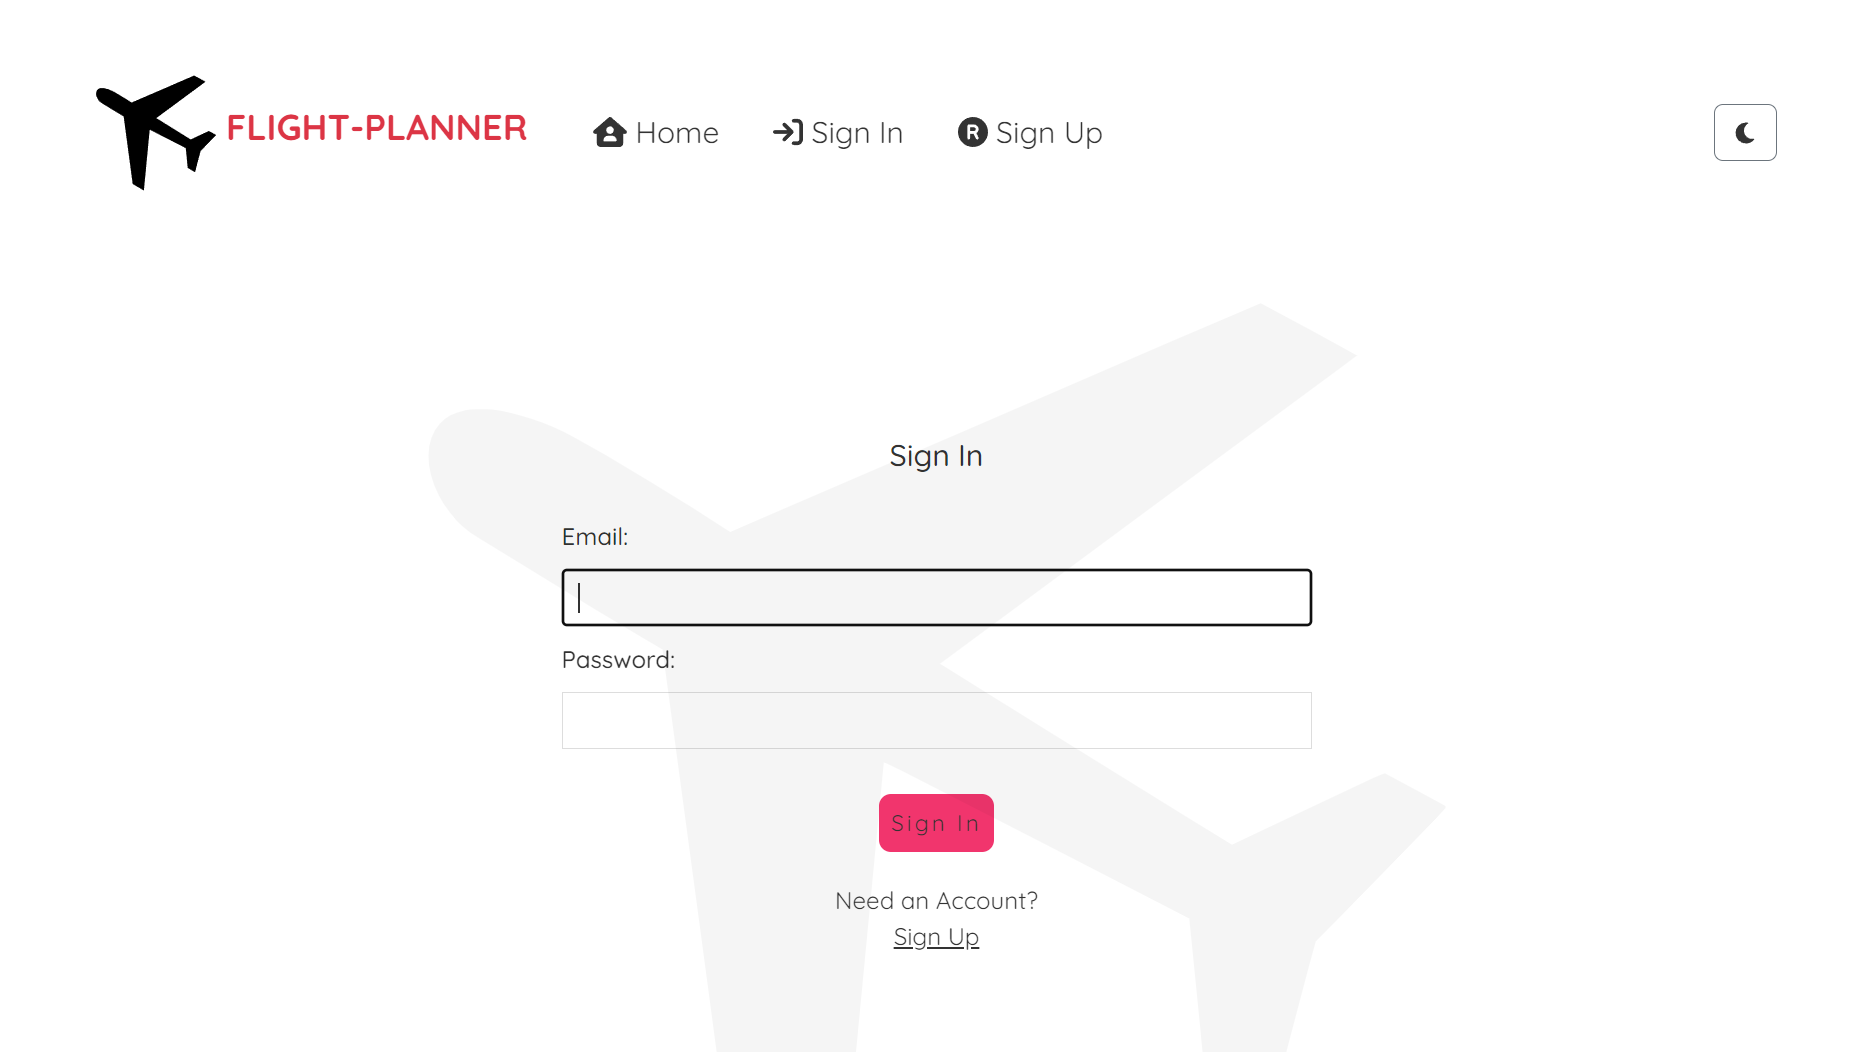
\includegraphics[width=0.6\linewidth]{1} 
    \caption{Formularz logowania}
\end{figure}
\begin{figure}[!ht]
    \centering
    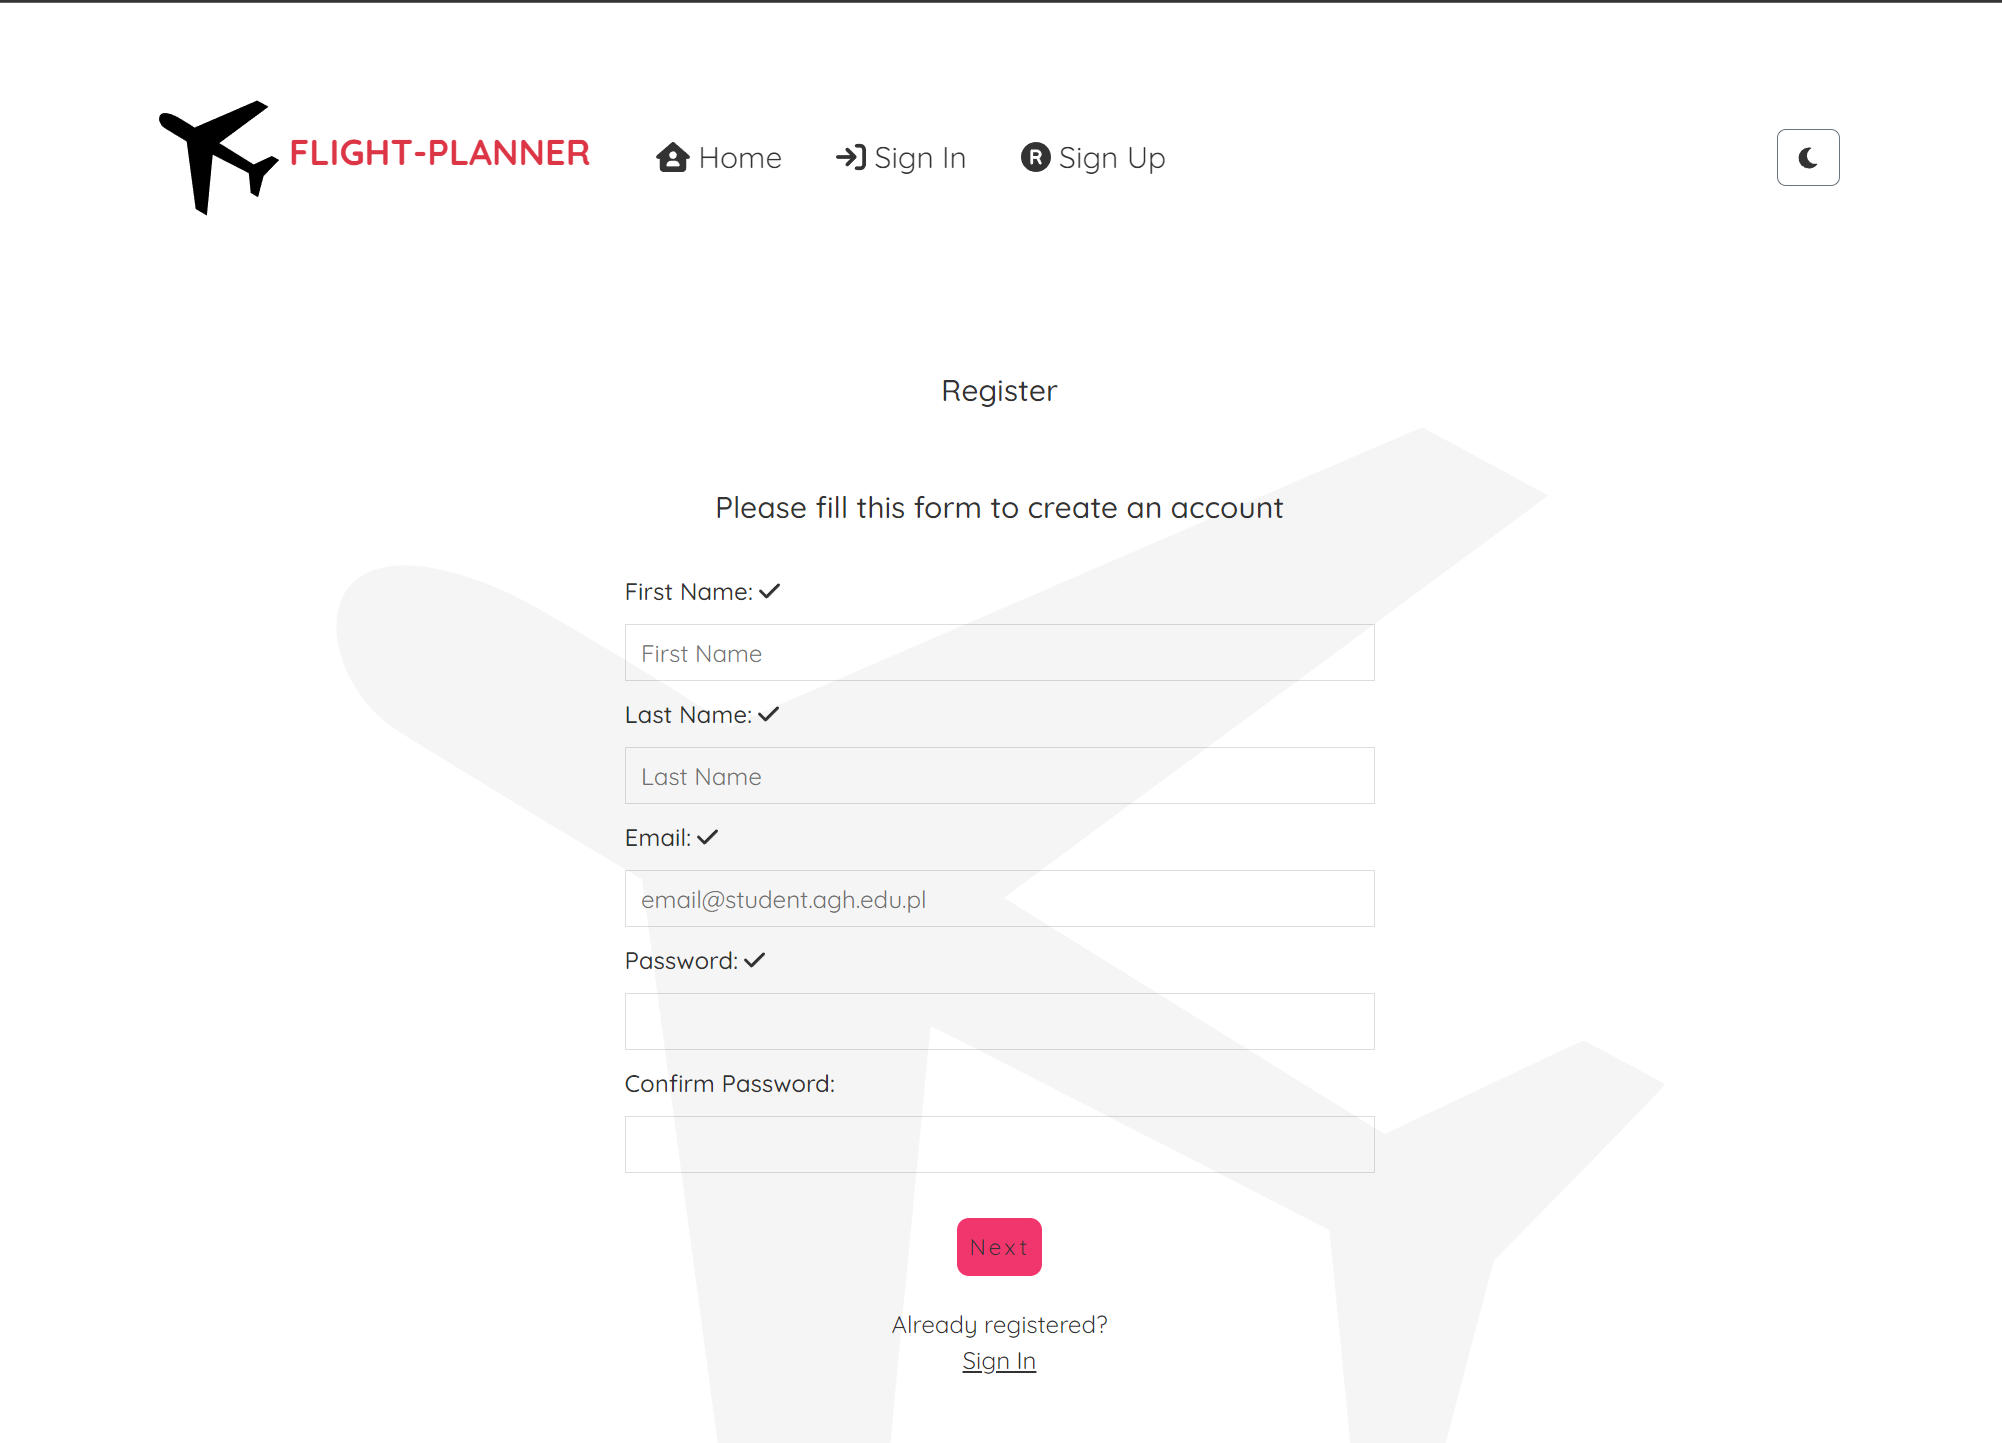
\includegraphics[width=0.7\linewidth]{2} 
    \caption{Formularz rejestracyjny}
\end{figure}
\newpage
Na górze ekranu znajduje się pasek nawigacji. Z jego poziomu, za pomocą rozwijanej opcji 'Add' można dodać nowe lotnisko. Opcja z kategorii 'Search' zwracaja listę połączeń między lotniskami oraz dostarcza możliwości znalezienia najkrótszej ścieżki pomiędzy określonymi miastami lub ścieżki z najmniejszą liczbą przesiadek.
W zakładce 'Add' $->$ 'Manage Airports' znajduje się lista wszystkich lotnisk z możliwością filtrowaniu po określonym kraju. Po kliknięciu odpowiedniej opcji ukazuje się nam 3 typy formularzy służą one do dodawania nowego lotniska jego edycji oraz dodania połączenia z innym lotniskiem. Posiadamy też możliwość usunięcia danego lotniska razem ze wszystkimi jego połączeniami.\\
\begin{figure}[!ht]
    \centering
    \begin{subfigure}{.95\textwidth}
        \centering
        
\includegraphics[width=0.7\linewidth]{4} 
        \caption{Formularz dodawania lotniska}
    \end{subfigure}
    \newline
    \begin{subfigure}{.45\textwidth}
        \centering
        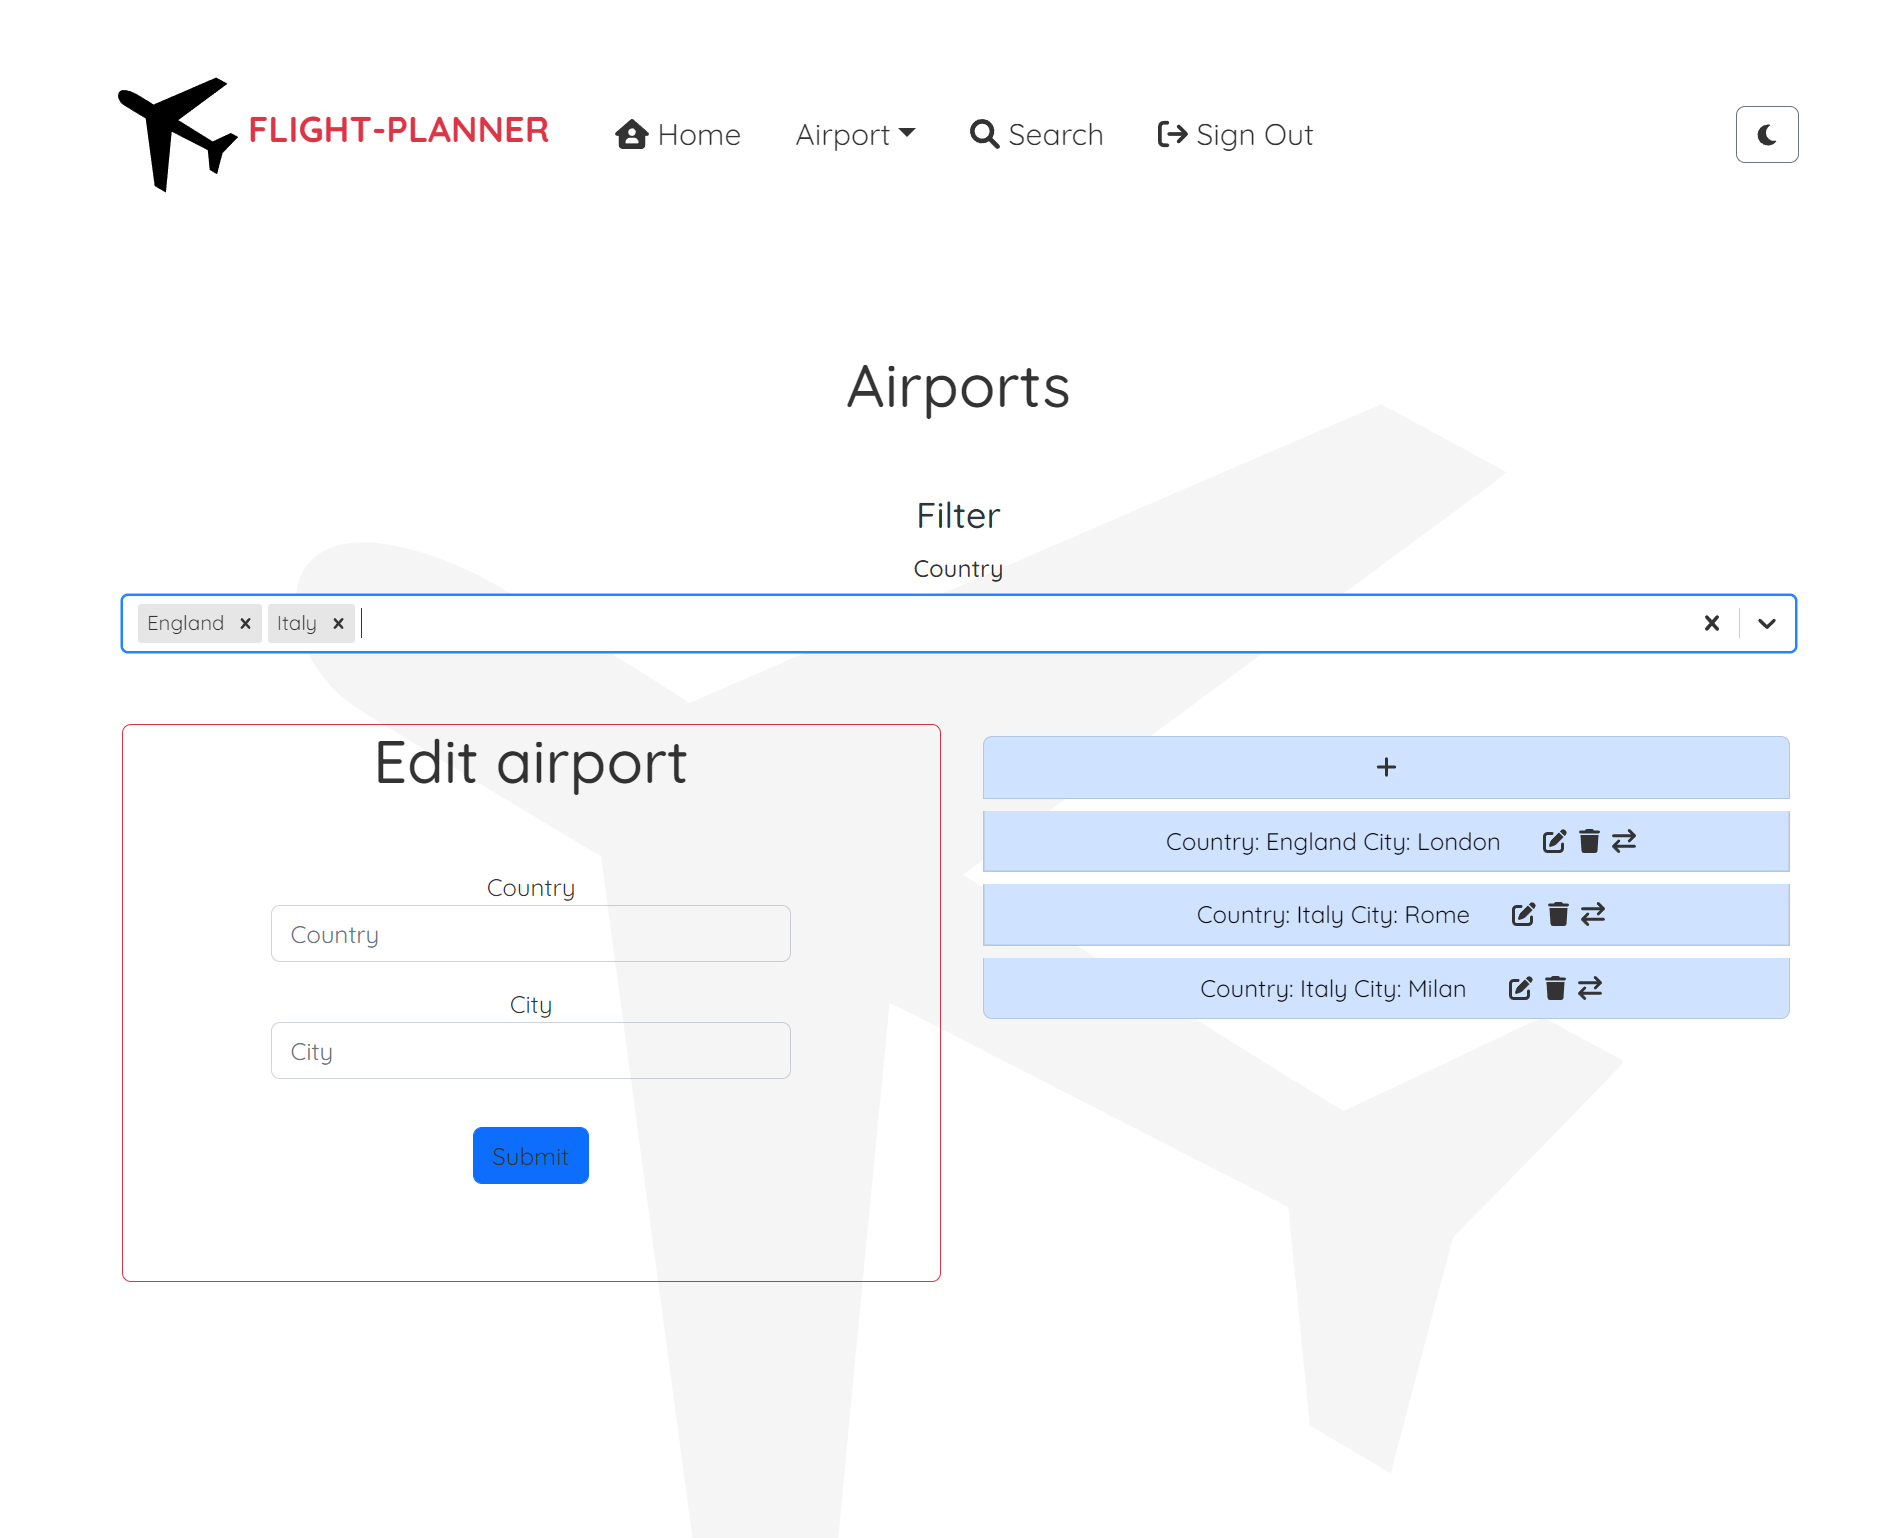
\includegraphics[width=0.95\linewidth]{5}  
        \caption{Formularz edycji lotniska}
    \end{subfigure}
    \begin{subfigure}{.45\textwidth}
        \centering
        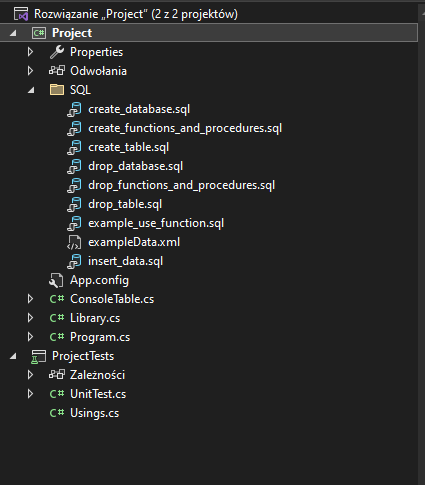
\includegraphics[width=0.95\linewidth]{6}  
        \caption{Formularz dodawania połączenia}
    \end{subfigure}
\end{figure}
\newpage
Tabela w zakładce "Connections" zwraca nam wszystkie połaczenia pomiedzy miastami aplikacja zapewnia nam możliwośc filtrowania i sortowania rekordów.\\
\begin{figure}[!ht]
    \centering
    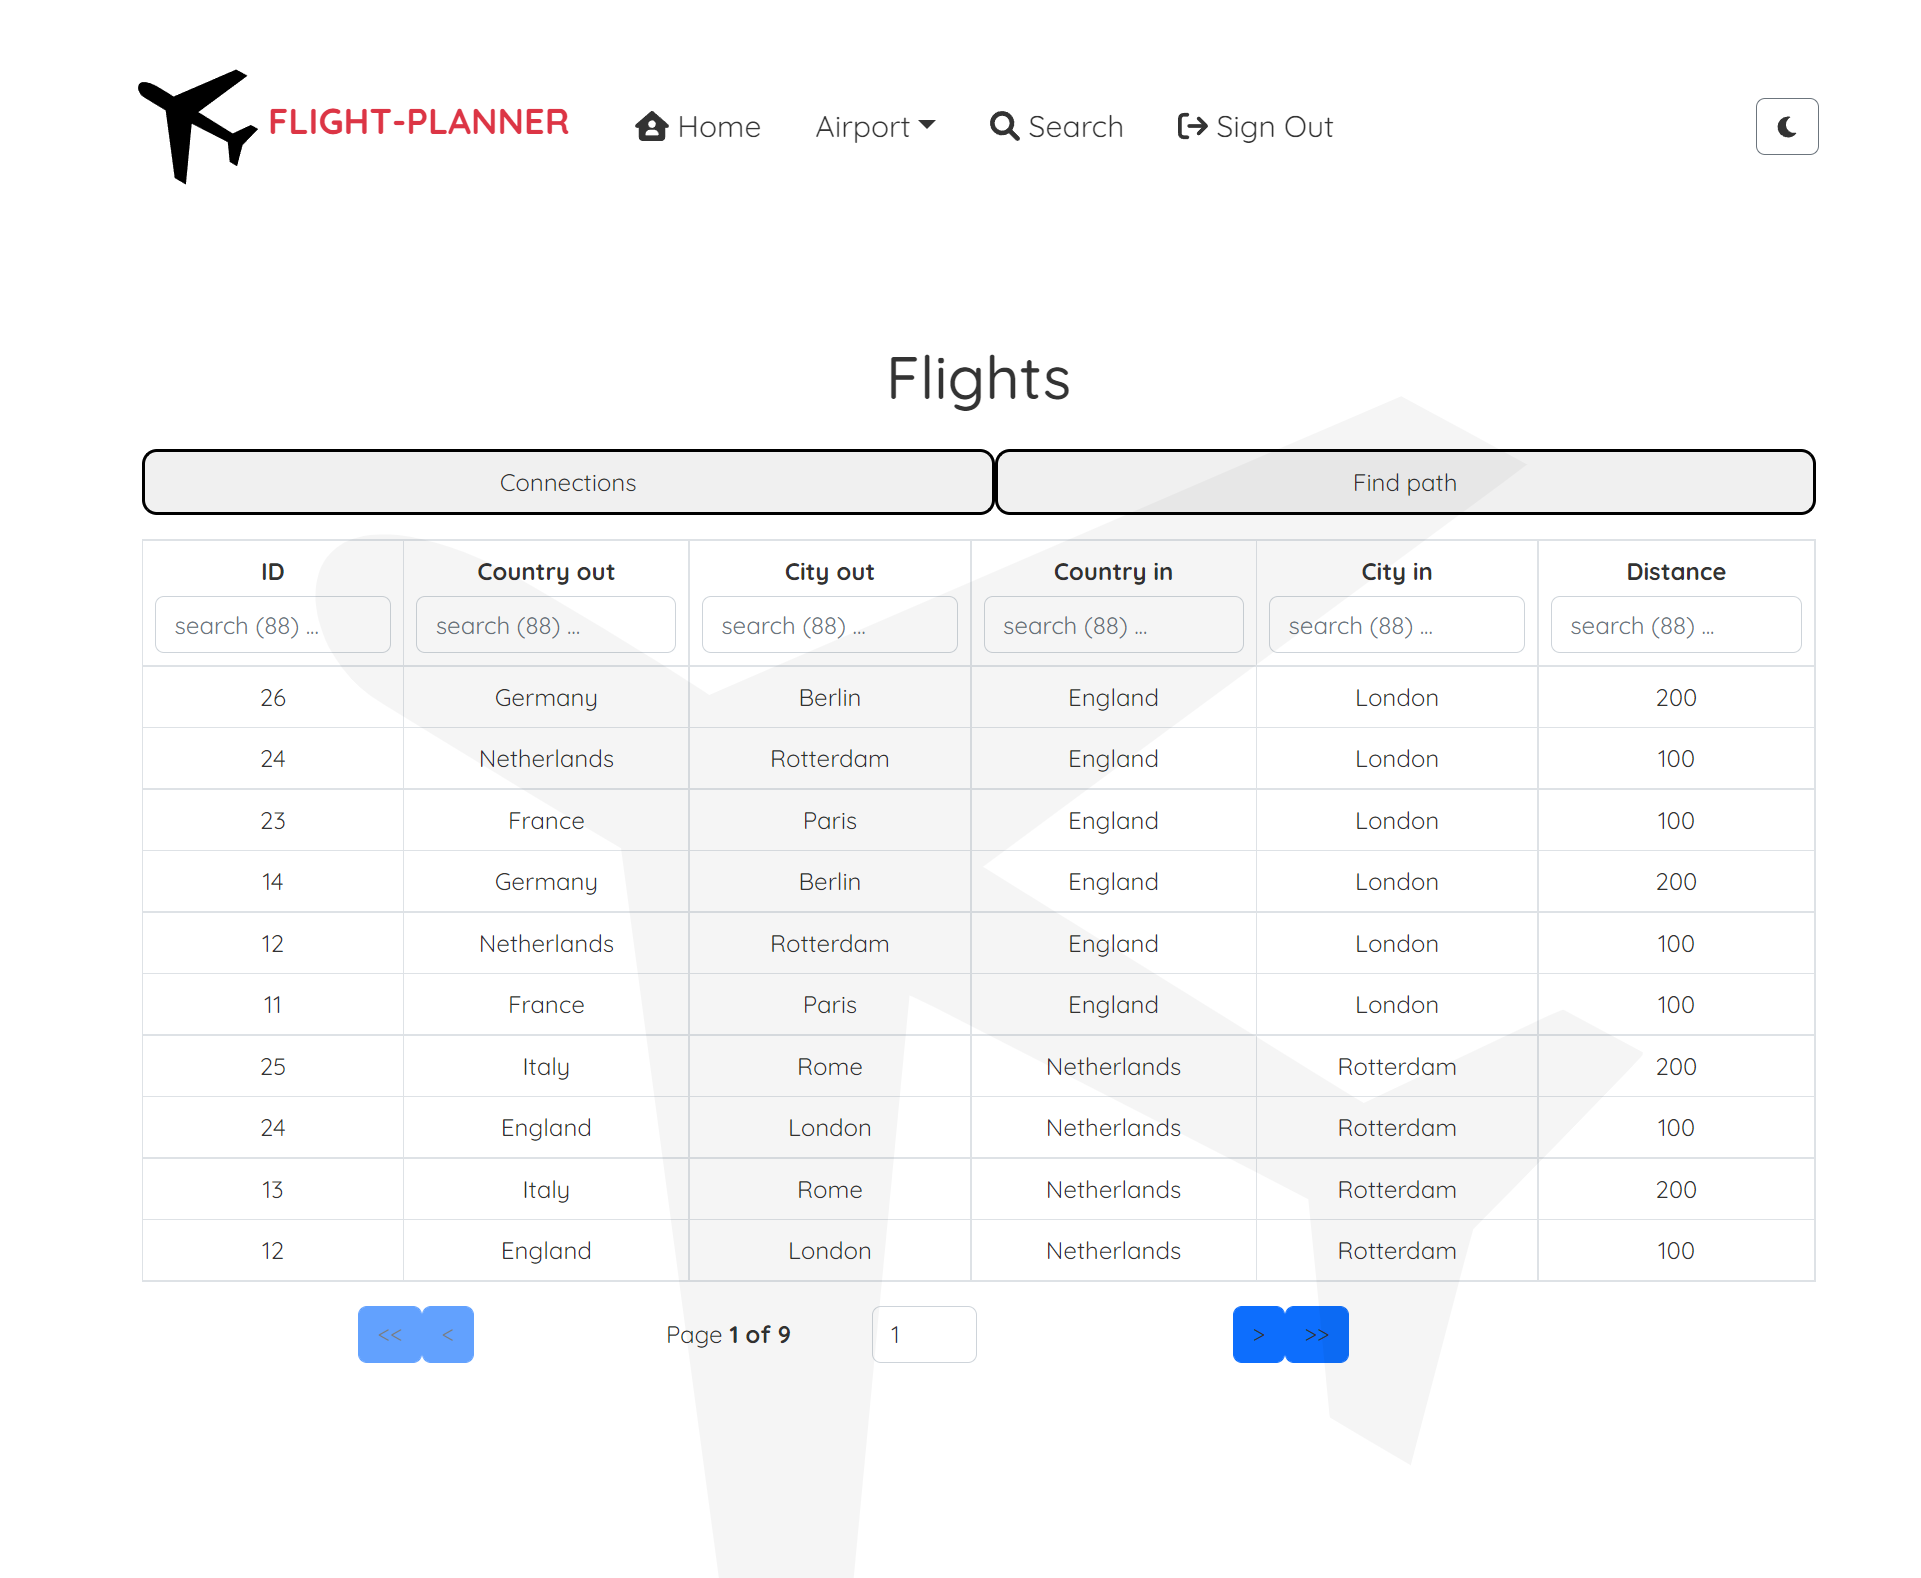
\includegraphics[width=0.55\linewidth]{7}  
    \caption{Menu z wyborem u}
\end{figure}
Tabela widoku "Find Path" ma jednakową formę dla każdego zapytania zwraca listę lotnisk, spełniające zadany warunek, w formie tabeli. Dla każdego lotniska zwracana jest id połaczenia nazwa kraju oraz miasta lotniska startowego oraz kraju i miasta celu podróży. Podana jest też estymowany dystans pomiedzy lotniskami.
Pierwszym wpisem jest lotnisko początkowe, natomiast kolejnymi są następujące po sobie przystanki, prowadzące do celu podróży.
Ostatnim wierszem w tabeli jest wybrany cel podróży
\begin{figure}[!ht]
    \centering
    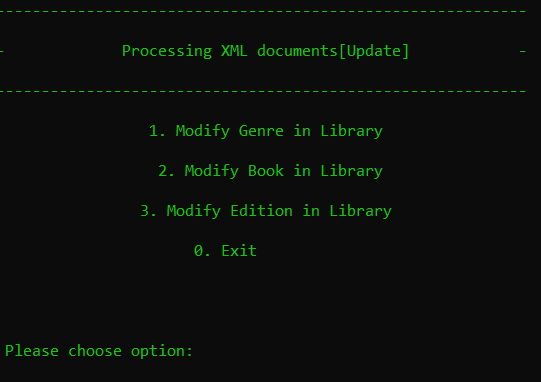
\includegraphics[width=0.55\linewidth]{8}  
    \caption{Menu z wyborem u}
\end{figure}
\newpage
\section{Wdrożenie aplikacji}
Aplikacje można uruchomić z pomocą kontenera utworzonego za pomocą pliku Dockerfile.\\
Wykonując komendę "docker-compose up -d" budujemy uprzednio obraz react-image (jeśli taki jeszcze nie istniał), następnie
kopiuje odpowiednie foldery z projektu, a następnie instalowane są potrzebne moduły komendą npm install. Potem budowana jest aplikacja reactowa komendą npm run build, a następnie odpalany jest server, który obsługuje komunikacje z bazą danych oraz wyświetla aplikacje posługując sie uprzedni zbudowanym klientem.\\
Czasami potrzebne jest przejście do folderu client i wykonać komende npm install oraz npm run build jeszcze raz
Aplikacja działa za pomocą kontenera Docker, ponieważ platformy takie jak Heroku czy IBM nie pozwalają już na bezpłatnością uruchomienie aplikacji na serwerze.

\section{Ewentualne usprawnienia możliwe do wykonania}
Aby usprawnić działanie aplikacji należy dodać o wiele więcej połączeń z dodatkowym parametrem daty lotu, a następnie wyszukiwać optymalnych połączeń ze względu na dystans liczbę przesiadek oraz godziny odlotu i przylotu\\
Do pełni funkcjonalności można też dodać dodatkowy rodzaj węzła, jakim jest samolot, a następnie przypinać/odpinać go od węzłów lotniska, jeśli wykonywane jest przelot z jednego lotniska na drugie.

\section{Literatura}
\begin{description}
\item {[1]} Antoni Dydejczyk, Przetwarzanie danych w chmurach obliczeniowych\\
\textit{https://newton.fis.agh.edu.pl/~antek/index.php?sub=dc\_wykl}
\item {[2]} Neo4j, Shortest path planning\\
\textit{https://neo4j.com/docs/cypher-manual/current/execution-plans/shortestpath-planning/}
\end{description}

\end{document}

